% EPL master thesis cover template
\documentclass{eplmastersthesis}

% Fill in here the information: title, student name, speciality, jury members
\title{Title of the master thesis}	% Master thesis title
\subtitle{Subtitle (optional)}			% Optional subtitle
\author{Zélie \textsc{Mulders}}	% Student name
% \secondauthor{Firstname \textsc{Lastname}}	% Second student name if applicable
\speciality{Computer Science and Engineering}		% Speciality (use one of the following options):
										% Biomedical Engineering
										% Chemical and Materials Engineering
										% Civil Engineering
										% Computer Science
										% Computer Science and Engineering
										% Electrical Engineering
										% Electro-mechanical Engineering
										% Mathematical Engineering
										% Mechanical Engineering
										% Physical Engineering
%\options{Option(s)}		% If required by program commission mention options
\supervisor{Kim \textsc{Mens}}	% 1st supervisor name
\cosupervisor{Philippe \textsc{Baret}}	% 2nd supervisor name if applicable
\cosupervisortwo{Adrien \textsc{Dockx}}
\readerone{Hélène \textsc{Verhaege}}		% 1st reader name
% \readertwo{Firstname \textsc{Lastname}}		% 2nd reader name
% \readerthree{Firstname \textsc{Lastname}}	% 3rd reader name
\years{2017-2018}	% Academic year

\usepackage{todonotes}
\usepackage{url}

\usepackage[tikz]{bclogo}
\usepackage[gen]{eurosym}
\usepackage{hyperref}
\usepackage{subcaption}

\begin{document}

\maketitle					% To create front cover page

\thispagestyle{empty}		% To suppress header and footer on the back of the cover page

\tableofcontents




\chapter{Introduction}
% 



\section{Context}
% Context: Sketch the context and domain of the work. 
\section{Problem}
% Problem:  Describe  and  define  the  problem  that  will  be 
% tackled in this thesis. 
\section{Motivation}
% Motivation: Motivate why this problem is a relevant one. 
% Why  is  this  problem  important,  complex,  not  yet  solved, 
% what are the shortcomings today. Optionally add a motiva-
% tion why you have chosen this particular thesis topic or why 
% this topic was proposed. 
\section{Objectives}
% Objectives: Highlight the intended objectives of your the-
% sis. What is the goal of this work? (In the conclusion chap-
% ter  you  will  come  back  to  these  objectives  and discuss  to 
% what extent you managed to achieve those objectives.) 
\section{Approach}
% Approach: Without going in full detail, present in general 
% terms how you will solve the problem and achieve the ob-
% jectives. 

\section{Contribution}
% Contributions:  Explicitly  highlight  the  major  and  minor 
% research contributions of your work. These can be of vari-
% ous kinds but it is important to stress the novel aspect; e.g.:  
%   identification  or  specification  of  a  new  relevant 
% problem; 
%   proposal  of  a  novel  solution  to  an  existing  prob-
% lem; 
%   new  mathematical  formalisms,  definitions,  theo-
% rems or proofs; 
%   design  of  a  novel  framework,  system,  language, 
% …; 
%   a  comparison  (or  survey)  of  existing  theories, 
% models, designs, systems or implementations in a 
% novel way;  
%   first implementation of a designed system significantly improved implementation of an existing 
% system); 
%   an  empirical  analysis,  for  example  a  study  of  the 
% performance of an implemented system; 
%   confirming  or  validation  of  the  correctness  of 
% someone  else’s  work  (for  the  first  time  or  in  a 
% novel way). 

\section{Roadmap}

% Roadmap:  Finish  this  section  by  announcing  how  the  re-
% mainder of your thesis document is structured, e.g.: 
% “The  remainder  of  this  document  is  structured  as 
% follows: the next two chapters provide the necessary 
% background  material  and  report  on  related  work. 
% Then, the proposed solution to the problem is intro-
% duced,  motivated,  defined  and  worked  out.  The 
% software architecture supporting the implementation 
% of that solution is then explained, and exemplified. 
% An  experiment/validation/case  study  is  then  con-
% ducted  in  order  to  validate  the  solution.  Finally,  a 
% conclusion  delivers  the  main  contributions  of  this 
% research  and  we  present  some  avenues  of  future 
% work.” 
% Hint: Try to phrase that roadmap paragraph in concrete terms 
% dedicated to your concrete problem and solution. If someone 
% else can just copy paste it and put it in his graduation thesis, 
% then you are probably not concrete enough. 


\chapter{Problem analysis in market gardening}
%\todo[inline]{In this chapter, we will describe the background of this master thesis. It contains all pieces of information needed to understand the thesis, even without any knowledge of the field processed.
%The background can be split between the two fields concerned by this master thesis. On the one hand, we have the background concerning the development of the application, related to the field of the software engineering. On the other hand, we can describe the background relative to the field of market gardening.}

In this chapter, we will talk about market gardening. It contains all pieces of information needed to understand the thesis, even without any knowledge of this field. We will also analyse this field and define different problems encountered during the management of a market gardening farm.

\section{Some vocabulary about market gardening}
First, it can be useful to define some common terms used in gardening.
\paragraph{Market gardening} A market gardener is someone who produces fruit and vegetables on a relatively small area. The difference between a farmer and a market gardener is principally in the type of final product. Where a farmer will produce more cereals, a market gardener is specialized in fruits and vegetables. We will use the term \emph{Truck farmers} for gardens that are cultivated with heavy machinery.  


\paragraph{Bed} A bed in a market garden is a surface of production, usually a line. It is used to divide the field in smaller cultivated areas. A picture of beds is shown on figure \ref{fig:beds}. Market gardener usually choose the width of their beds according to the width of the tools they are going to use.

\begin{figure}
    \centering
    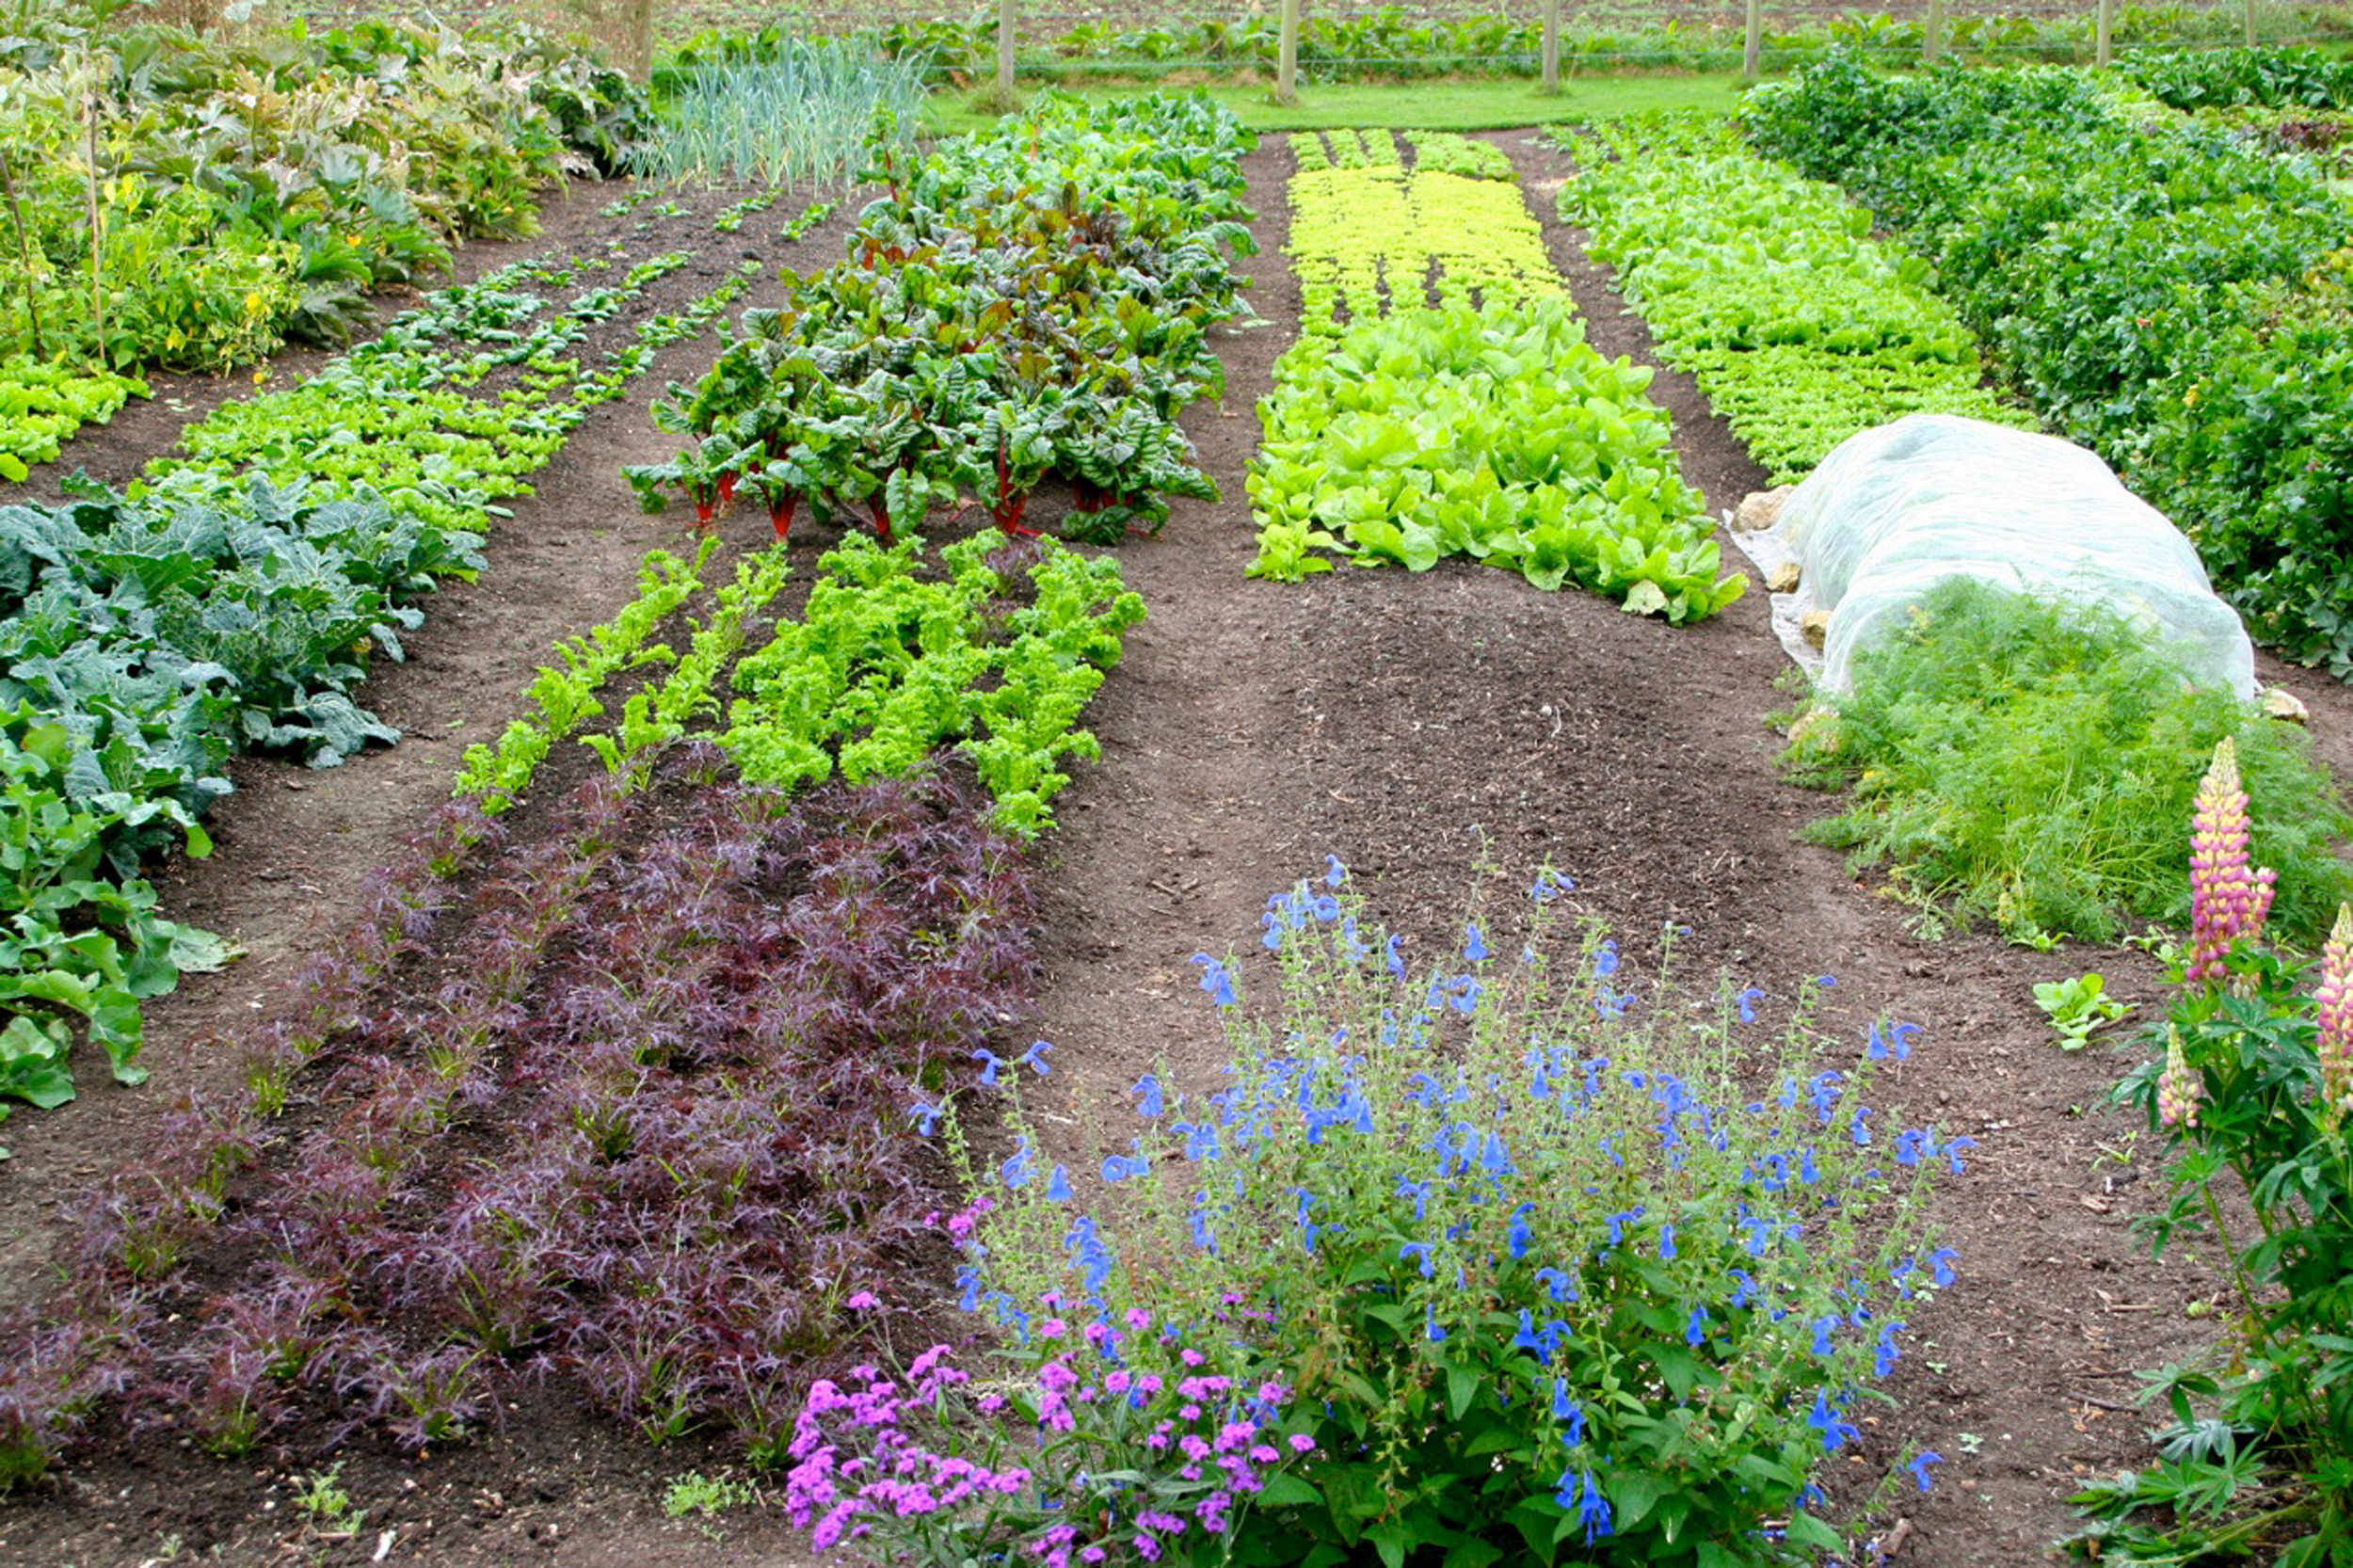
\includegraphics[width=0.6\textwidth]{images/beds.jpg}
    \caption{Beds in a market garden}
    \label{fig:beds}
\end{figure}

\paragraph{Crop rotation} In order to preserve the soil from draining and to eliminate some diseases specific to some plant species, some market gardener rotate their cropping. If they plant one type of vegetable on a bed, the year after they will plant another type of vegetable on this bed. They will not plant two years in a row the same vegetable on the same bed.

\section{Daily life scenario}

\paragraph{Seasons} Market gardeners live by the rhythm of the seasons: they have a peak of work during the Spring and the Summer. Harvests continue during Autumn but during Winter they usually have less things to do in the garden. 

\paragraph{Planning}

Most gardeners plan their cropping during winter\cite{planification-methodology}, when they have more time to think about what they want to grow this year. Planning the coming year has several advantages : 

\begin{itemize}
	\item Know in advance what amounts of seeds and fertilizers they will have to order
	\item Take the time to decide what to grow and in what quantities
	\item Look back at the previous year to see which vegetables were the most profitable and adjust cropping according to this experience.
	\item Gain time during the rush season by having clearly in mind what has to be done
	\item Organise the year to spread the work as most as possible (everything can not be seeded the same week)
\end{itemize}

While really useful, this planning part is not always done by market gardeners. 

\paragraph{Adaptations}
Once the work season has started, this planning has to be adapted to the reality on the ground.
The weather is the major factor of changes in the planning. Indeed, some seeding requires several days of dry weather followed by one day of rain for example. In the case of difficult weather (late frost, large humidity,...), whatever was the initial plan, the gardener will have to adapt his schedule to the weather.
Others factors that disrupt the work set-up can be diseases in the crops, short staffing or hardware issues.
One example scenario could be:
We are the first week of July, the season is in full swing. Tim is a market gardener and had planned to plant endives this week. The weather conditions are perfect, so he could stick to his plan. Unfortunately, his tomatoes have mildew\footnote{an epidemic fungus  \url{https://en.wikipedia.org/wiki/Mildew}} and if he wants to save his tomatoes' crops, he has to treat them immediately.

This example shows that some events have priority over the initial plan and confirm the idea that initial planning is meant to evolve.

It is essential for a market garden to be able to adapt its plans to a specific situation and to keep a clear head as we go along the season. Planning is already not and easy task, but adapting to changes is even harder. 



\section{Profitability of market gardens}


% These antoinette dumont
%\begin{itemize}
%\item difficile d'estimer les couts unitaires:
%\item difficile d'estimer combien rapporte chaque légume
%\item difficile de savoir combien de temps passer sur chaque culture et donc de savoir laquelle est la plus profitable.
%\end{itemize}
%
%
%


\paragraph{Workforce} Market gardeners don't count their hours as regular workers. They work all day in order to reach their objectives of the day. Most of them have no idea of how long each culture takes. It also means that they have no idea how profitable their cultures are. Moreover, they often need external workers to help them during the peak season. These external workers represent 50\% of productions costs \cite{fortier}. Consequently, organizing the work to reduce the need of external workers can have a considerable impact on the garden's profitability.

\paragraph{Vegetables profitability}
Some vegetables are more profitable than others. For example, Jean-Martin Fortier \cite{fortier} in his book gives data about the profitability of the vegetables he's growing. However, most farmer don't do this analysis on their production and have therefore, no idea of which cropping is the most profitable. Even in the table of Jean-Martin Fortier, we have no idea of the work time needed for each culture. And yet we have seen before that workforce represent a significant cost.
Moreover, from one area to another it is reasonable to think that some crops will be more profitable than others. Depending on the clients' preferences or the soil type, some vegetables will be easier to sell or to crop.
Gardeners are mostly not analysts and don't have the right tools to give them an idea of how profitable their business is and how they could be more efficient.

\paragraph{Others profitability factors}

\begin{itemize}
\item Retail strategy: different retails strategies will give different revenues, the more intermediaries there are between the producer and the client, the less the producer will gain.
\item Pricing strategy: of course, the selling price of vegetables will affect the profitability of this vegetables. Depending on which retail strategy is chosen, prices will be more or less flexible.
\end{itemize}

Antoinette Dumont has dedicated her doctoral thesis on the subject of market gardens' profitability.\cite{adumont}

\section{Researches in gardening}

\todo[inline]{Complete this section}

\section{Existing tools}

From our researches, there is not a lot of software to help farmers of all kind in their daily life. Furthermore, most of them are not open source.

First, we found software like \emph{Mes petits légumes}\cite{mespetitslegumes} intended for non-professional market gardeners, with a great library of data about lots of vegetables. The software can be bought once for 19 \euro{} or one can use the free incomplete version. Two screenshots of this application are shown on image \ref{fig:mespetitslegumes}

\begin{figure}
\centering
\begin{subfigure}{.5\textwidth}
  \centering
  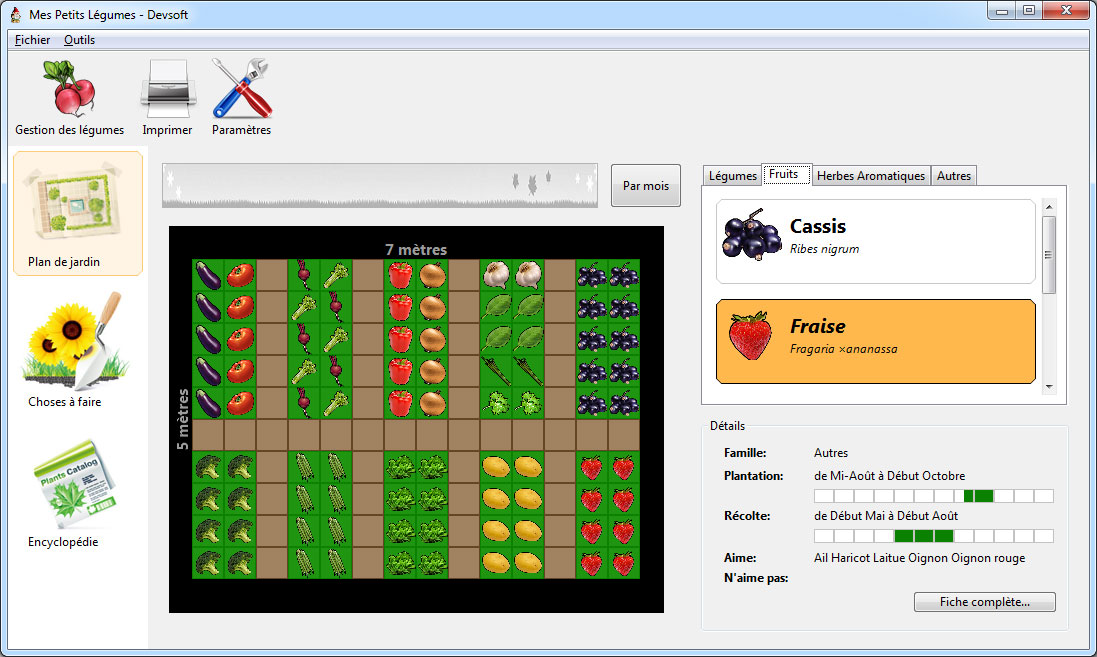
\includegraphics[width=0.9\linewidth]{images/petitslegumes1.jpg}
  \caption{Visual representation of a garden planning}
  \label{fig:petitslegumes1}
\end{subfigure}%
\begin{subfigure}{.5\textwidth}
  \centering
  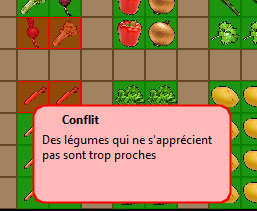
\includegraphics[width=0.7\linewidth]{images/petitslegumes2.jpg}
  \caption{Intercropping advices}
  \label{fig:petitslegumes2}
\end{subfigure}
\caption{Screenshots of the software \emph{Mes petits légumes}}
\label{fig:mespetitslegumes}
\end{figure}



Then, we have softwares like \emph{LEA}\cite{lea-agri} more focused on the management of the business and intended for big farms. It can generate bill from tractor work. It helps managing stocks and uses of fertilizers. 
Once again, the software is not open source and a subscription is required to use it.

Finally, we have found a software that seems to have a purpose and a target audience similar to this project. \emph{Tend}\cite{tend} is a software developed in the USA by a Startup. It has lots of features, including a databases of vegetables, a task calendar and an expenses section. The main feature (constitute a crop plan by adding plantings) is shown on figure \ref{fig:tend}.

\begin{figure}
\centering
\begin{subfigure}{.5\textwidth}
  \centering
  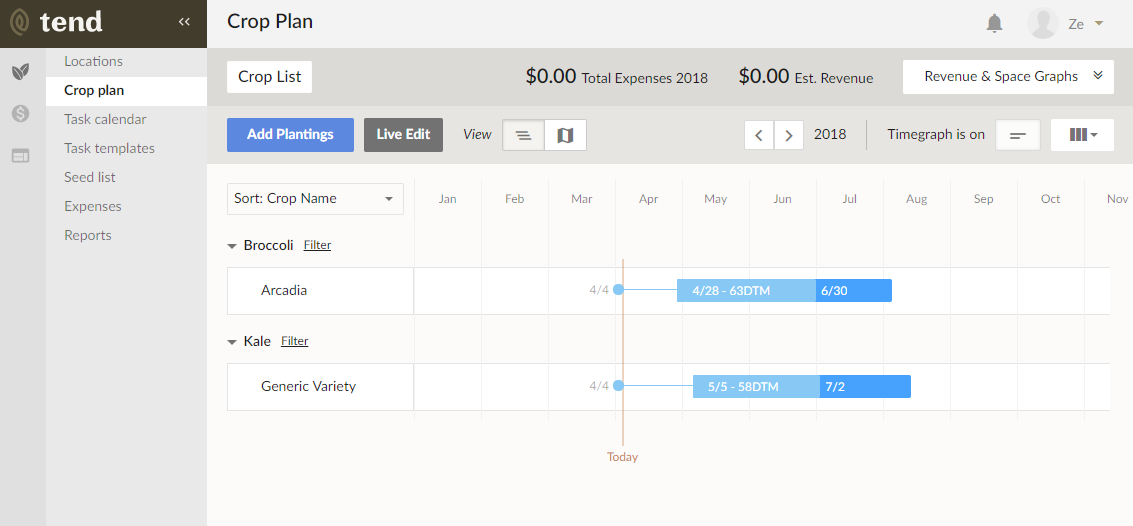
\includegraphics[width=0.9\linewidth]{images/tend1.PNG}
  \caption{Planning view}
\end{subfigure}%
\begin{subfigure}{.5\textwidth}
  \centering
  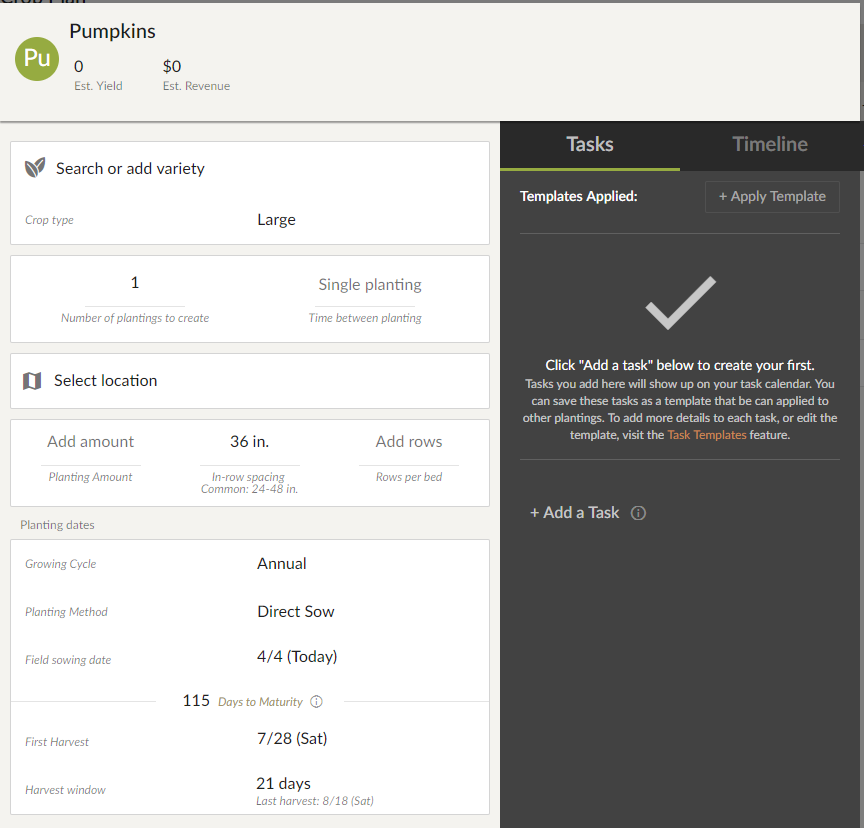
\includegraphics[width=0.7\linewidth]{images/tend2.PNG}
  \caption{Adding a new plantation}
\end{subfigure}
\caption{Screenshots of the software \emph{Mes petits légumes}}
\label{fig:tend}
\end{figure}

These software show that farmers are in need of tools to help them in their planning and management. The poorness of software really adapted to their needs show that this field has been forgotten by technology.


\section{Conclusion}

From this analysis of the field of market gardening, 
\todo[inline]{+ say that this is where this thesis comes in}

\chapter{Problem analysis in software engineering}
\todo[inline]{For each thing you explain also say why you explain it, what role will it play later in this thesis}

\section{In computer science and in software engineering}
\paragraph{Agile Methodology}
The Agile methodology is a set of techniques and principles for conducting a development project. The main principle is to iterate over short periods (called sprints) divided in subphases in order to build the final product in an incremental way.
A sprint lasts between one and two weeks and is divided as follows: 
\begin{itemize}
    \item At the start of each iteration, we plan with the client what we are going to do this iteration.
    \item Next step is to think about how to build a good design to achieve the objective
    \item Then, we develop the features
    \item After, we test these features. If we switch these last two steps, we apply what is called Test-Driven Development. With this methodology, a team write tests before developing the corresponding features, ensuring that the tests will cover all the cases
    \item At the end of each sprint, we meet the client again to validate the changes and new features, collect his feedback about the project's progress and to define together the future work.
\end{itemize}
A visual representation of this iterative approach is shown on figure \ref{fig:agile-methodology}


\begin{figure}
    \centering
    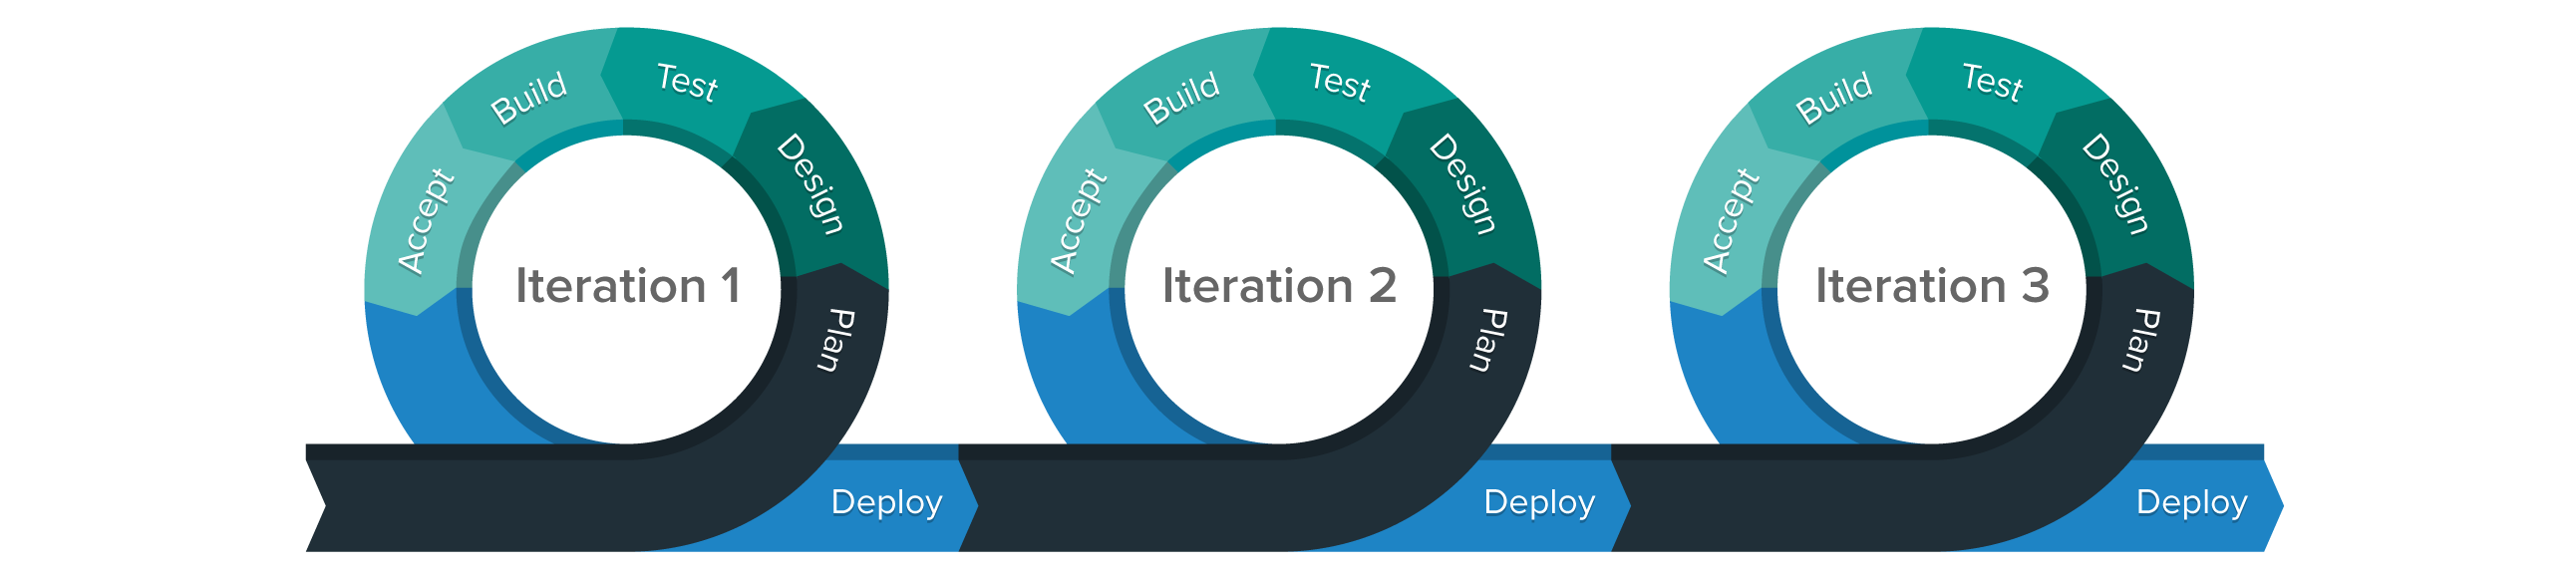
\includegraphics[width=\textwidth]{images/agile-methodolody.png}
    \caption{Iterations using Agile methodology}
    \label{fig:agile-methodology}
\end{figure}

A good summary of the Agile methodology is the agile manifesto\cite{agilemanifesto}, that states the main principles of this methodology.

\begin{bclogo}[logo=\bctrombone]{Agile Manifesto \cite{agilemanifesto}}
\emph{Individuals and interactions} over processes and tools.\\
\emph{Working software} over comprehensive documentation.\\
\emph{Customer collaboration} over contract negotiation.\\
\emph{Responding to change} over following a plan. \\
That is, while there is value in the items on
the right, we value the items on the left more.
\end{bclogo}

The main advantages of this methodology are to have flexibility and regular feedback on the product delivered.

\paragraph{Python}
Python is a programming language used in many fields. Its main advantage is great readability.

\todo[inline]{Talk more about python? Creator, specificity's, interpreted language, speed, community, TIOBE Index...? \url{ https://www.tiobe.com/tiobe-index/} Mainly explain why you chose it and what its main features/specificities you will rely upon}

\paragraph{Software framework}

A framework is a set of tools that provides features that can be reused in multiple applications. A framework is different from a library in the sense that when using a library, we call the methods of the library while when using a framework, our code is called by the framework. The difference is shown on figure \ref{fig:framework-vs-library}. Frameworks help to build reusable and maintainable applications 
\todo[inline]{give some examples of frameworks + why you talk about it, integrate Django with it?}

\begin{figure}
    \centering
    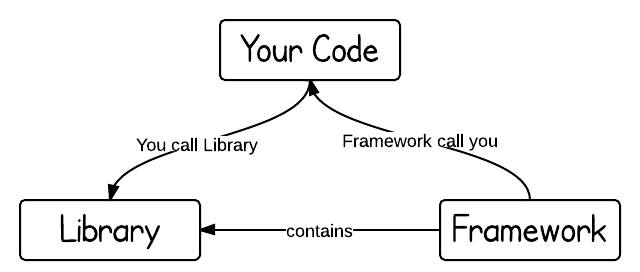
\includegraphics[width=0.5\textwidth]{images/framework-vs-library.png}
    \caption{Framework versus library}
    \label{fig:framework-vs-library}
\end{figure}
\paragraph{Django}
Django is a web framework to develop web applications in Python. 
\todo[inline]{Develop, why django, what others, what features of Djangos do you rely upon, what plugins, and so on}

\paragraph{Continuous Integration}
Continuous integration (often referred as CI) is a software engineering practice to help development teams working on a set repository. 
When using CI, we automate a set of checks at each push request on a repository and developers should merge to this repository regularly. With continuous integration, we will detect bugs faster and more easily. We can also add tests to our continuous integration tool, these tests will then be run at each push request and we will receive a notification if they fail. Thanks to that, we can see exactly which commit implied a failure in the tests. If we do small regular commits, it will be really easy to find where the failure comes from.

\todo[inline]{Why you explain this, what CI you use, what CI features and tools you use; why you use these}

\chapter{Solution}
% % Now  that  you  have  introduced  the  necessary  background 
% material  and  related  work,  you  can  explain  in  more  detail 
% the research problem that you want to address in this thesis, 
% why it is a relevant problem and how your solution would 
% advance the state of the art in this research area (by posi-
% tioning it in terms of the related work discussed in the pre-
% vious chapter). 

% Solution 
% In this chapter (or chapters), you describe in detail the solu-
% tion you have developed to address the problem. This chap-
% ter may be decomposed in several chapters describing dif-
% ferent  aspects  of  your  solution.  For  example,  one  chapter 
% introducing  a  new  formalism  you  developed,  another  de-
% scribing a novel algorithm you propose based on that for-
% malism,  and  finally  a  chapter  discussing  a  prototype  im-
% plementation of that algorithm. 
% What is most important to make clear in these chapters is 
% the conceptual ideas behind the solution. Try to describe the 
% essence of your solution so that any reader can understand 
% it,  even  though  you  can  add  some  more  detailed  sections 
% that  dive  into  the  technical  intricacies  of  the  solution  as 
% well.  A  reader  who  is  only  interested  in  the  big  picture 
% should be able to skip those more detailed sections and still 
% understand what your solution is about. A reader who wants 
% to understand your solution in full detail can decide to read 
% them. 
% Where  necessary,  provide  schemas  or  pictures  illustrating 
% how your solution works. A (good) picture often tells more 
% than  a  thousand  words.  Throughout  this  chapter,  illustrate 
% the different aspects of your solution on the running exam-
% ple. At the end of the chapter, don’t forget to position your 
% particular solution to the related work discussed in a previ-
% ous chapter.  

% \chapter{Analysis and methodology}
% \section{Analysis}



\section{Methodology}

We choose to use a Agile methodology because the requirements were not well established at the start of the master thesis. By using this development methodology, we were able to change and add requirements every week, giving us more flexibility. In this case, we had two different clients:
\begin{itemize}
    \item \textbf{UCL}: the University has bought a farm where they want to experiment different market gardening type and gather data. 
    \item \textbf{Farmers}: We wanted the app to be useful not only for the university, but also for farmers in their daily life. This approach is complementary as data from farmers are useful for university's researchers.
\end{itemize}
We add several meetings with farmers at the very beginning to define the problem, their expectations and their needs

\todo[inline]{Agile parce que redéfinition régulière du probleme}

\section{Tools and Technology}

\begin{itemize}
    \item choix de Python et Django, justification
    \item Trello pour l'organisation agile des taches
    \item Github pour projet open source et versionning
    \item Travis pour continuous integration
    \item CodeClimate pour qualité du code et test coverage
\end{itemize}



\chapter{Architecture}
% \begin{itemize}
    \item Diagrammes: uml, class, sequences,...
\end{itemize}

\todo[inline]{dessin pour la fac agro, dessin "vulgarisé" de l'utilsiation de l'application}

\chapter{Implementation}
% \begin{itemize}
    \item Constraint programming? Spécificités du prjet au niveau implémentation
\end{itemize}
\todo[inline]{Librairie de légumes implémentée en dupliquant les modèles mais dans une app différente}

\chapter{Validation}
% % In this chapter, describe the experiment, benchmarks, case 
% study or other means of validation, which you conducted to 
% prove that your solution attains the objectives put forward 
% in the introduction. 
\begin{itemize}
    \item Déploiemennt, partage à des maraichers : tests "humain"
    \item Tests unitaires, selenium, manuels
\end{itemize}

\chapter{Conclusion and future work}
% % Summarize the main findings of your work: what did you 
% do, what was not covered, advantages, shortcomings, pos-
% sible future work. Did you attain the initial objectives of the 
% thesis? 
% Make  sure  to  revisit  the  initial  problem  statement  and  to 
% point  out  explicitly  how  your  solution  addresses  it.  Also 
% repeat the achieved contributions. 

% FUTURE WORK 
% Discuss possible paths of future work here. A good idea is 
% to fill in this section throughout the entire year you work on 
% this thesis. Whenever you have a cool idea, put it here. If 
% you don’t have time to develop it, it becomes future work.  

\begin{itemize}
    \item Reprise par la fac Agro
    \item Objectifs atteints? Contraintes?
    \item Ajout de nouvelles fonctionnalités: application facilement extensible : pouvoir ajouter de la culture associée, pouvoir ajouter des photos, pouvoir ajouter un système de planification, ajouter une estimation des revenus (ce que rapporte chaque légume)...
\end{itemize}



\nocite{*} %pour qu'il affiche meme les non citées % BIEN JOUÉ =D
\bibliographystyle{plain}
\bibliography{biblio}

% Back cover page
\backcoverpage
\end{document}
